\documentclass{beamer}
\usepackage[orientation=portrait,size=a1,scale=1.4,debug]{beamerposter}
\mode<presentation>{\usetheme{ZH}}
\usepackage{chemformula}
\usepackage[utf8]{inputenc}
\usepackage[german, english]{babel} % required for rendering German special characters
\usepackage{siunitx} %pretty measurement unit rendering
\usepackage{hyperref} %enable hyperlink for urls
\usepackage{ragged2e}
\usepackage[font=scriptsize,justification=justified]{caption}
\usepackage{array,booktabs,tabularx}
\usepackage{multicol,multirow}

\newcolumntype{Z}{>{\centering\arraybackslash}X} % centered tabularx columns
\sisetup{per=frac,fraction=sfrac}

\title{\huge Vehicles Chasing Each Other \\Around a Closed Path}
\author{Erdem Tuna, Halil Temurtaş, Sarper Sertel, Enes Taştan, İlker Sağlık}
\institute[ETH]{$^{1}$Department of Electrical and Electronics Engineering, Middle East Technical University% \\ $^{2}$Preclinical Laboratory for Translational Research into Affective Disorders, DPPP, Psychiatric Hospital, University of Zurich
}
\date{March 1, 2019}

% edit this depending on how tall your header is. We should make this scaling automatic :-/
\newlength{\columnheight}
\setlength{\columnheight}{71cm}

\begin{document}
\begin{frame}
\begin{columns}
	\begin{column}{.5\textwidth}
		\begin{beamercolorbox}[center]{postercolumn}
			\begin{minipage}{.98\textwidth}  % tweaks the width, makes a new \textwidth
				\parbox[t][\columnheight]{\textwidth}{ % must be some better way to set the the height, width and textwidth simultaneously
					\begin{myblock}{Company and Shareholders}
BB

						\vspace{0.4em}
						\begin{figure}
							%\begin{minipage}{0.43\textwidth}
								\centering
								%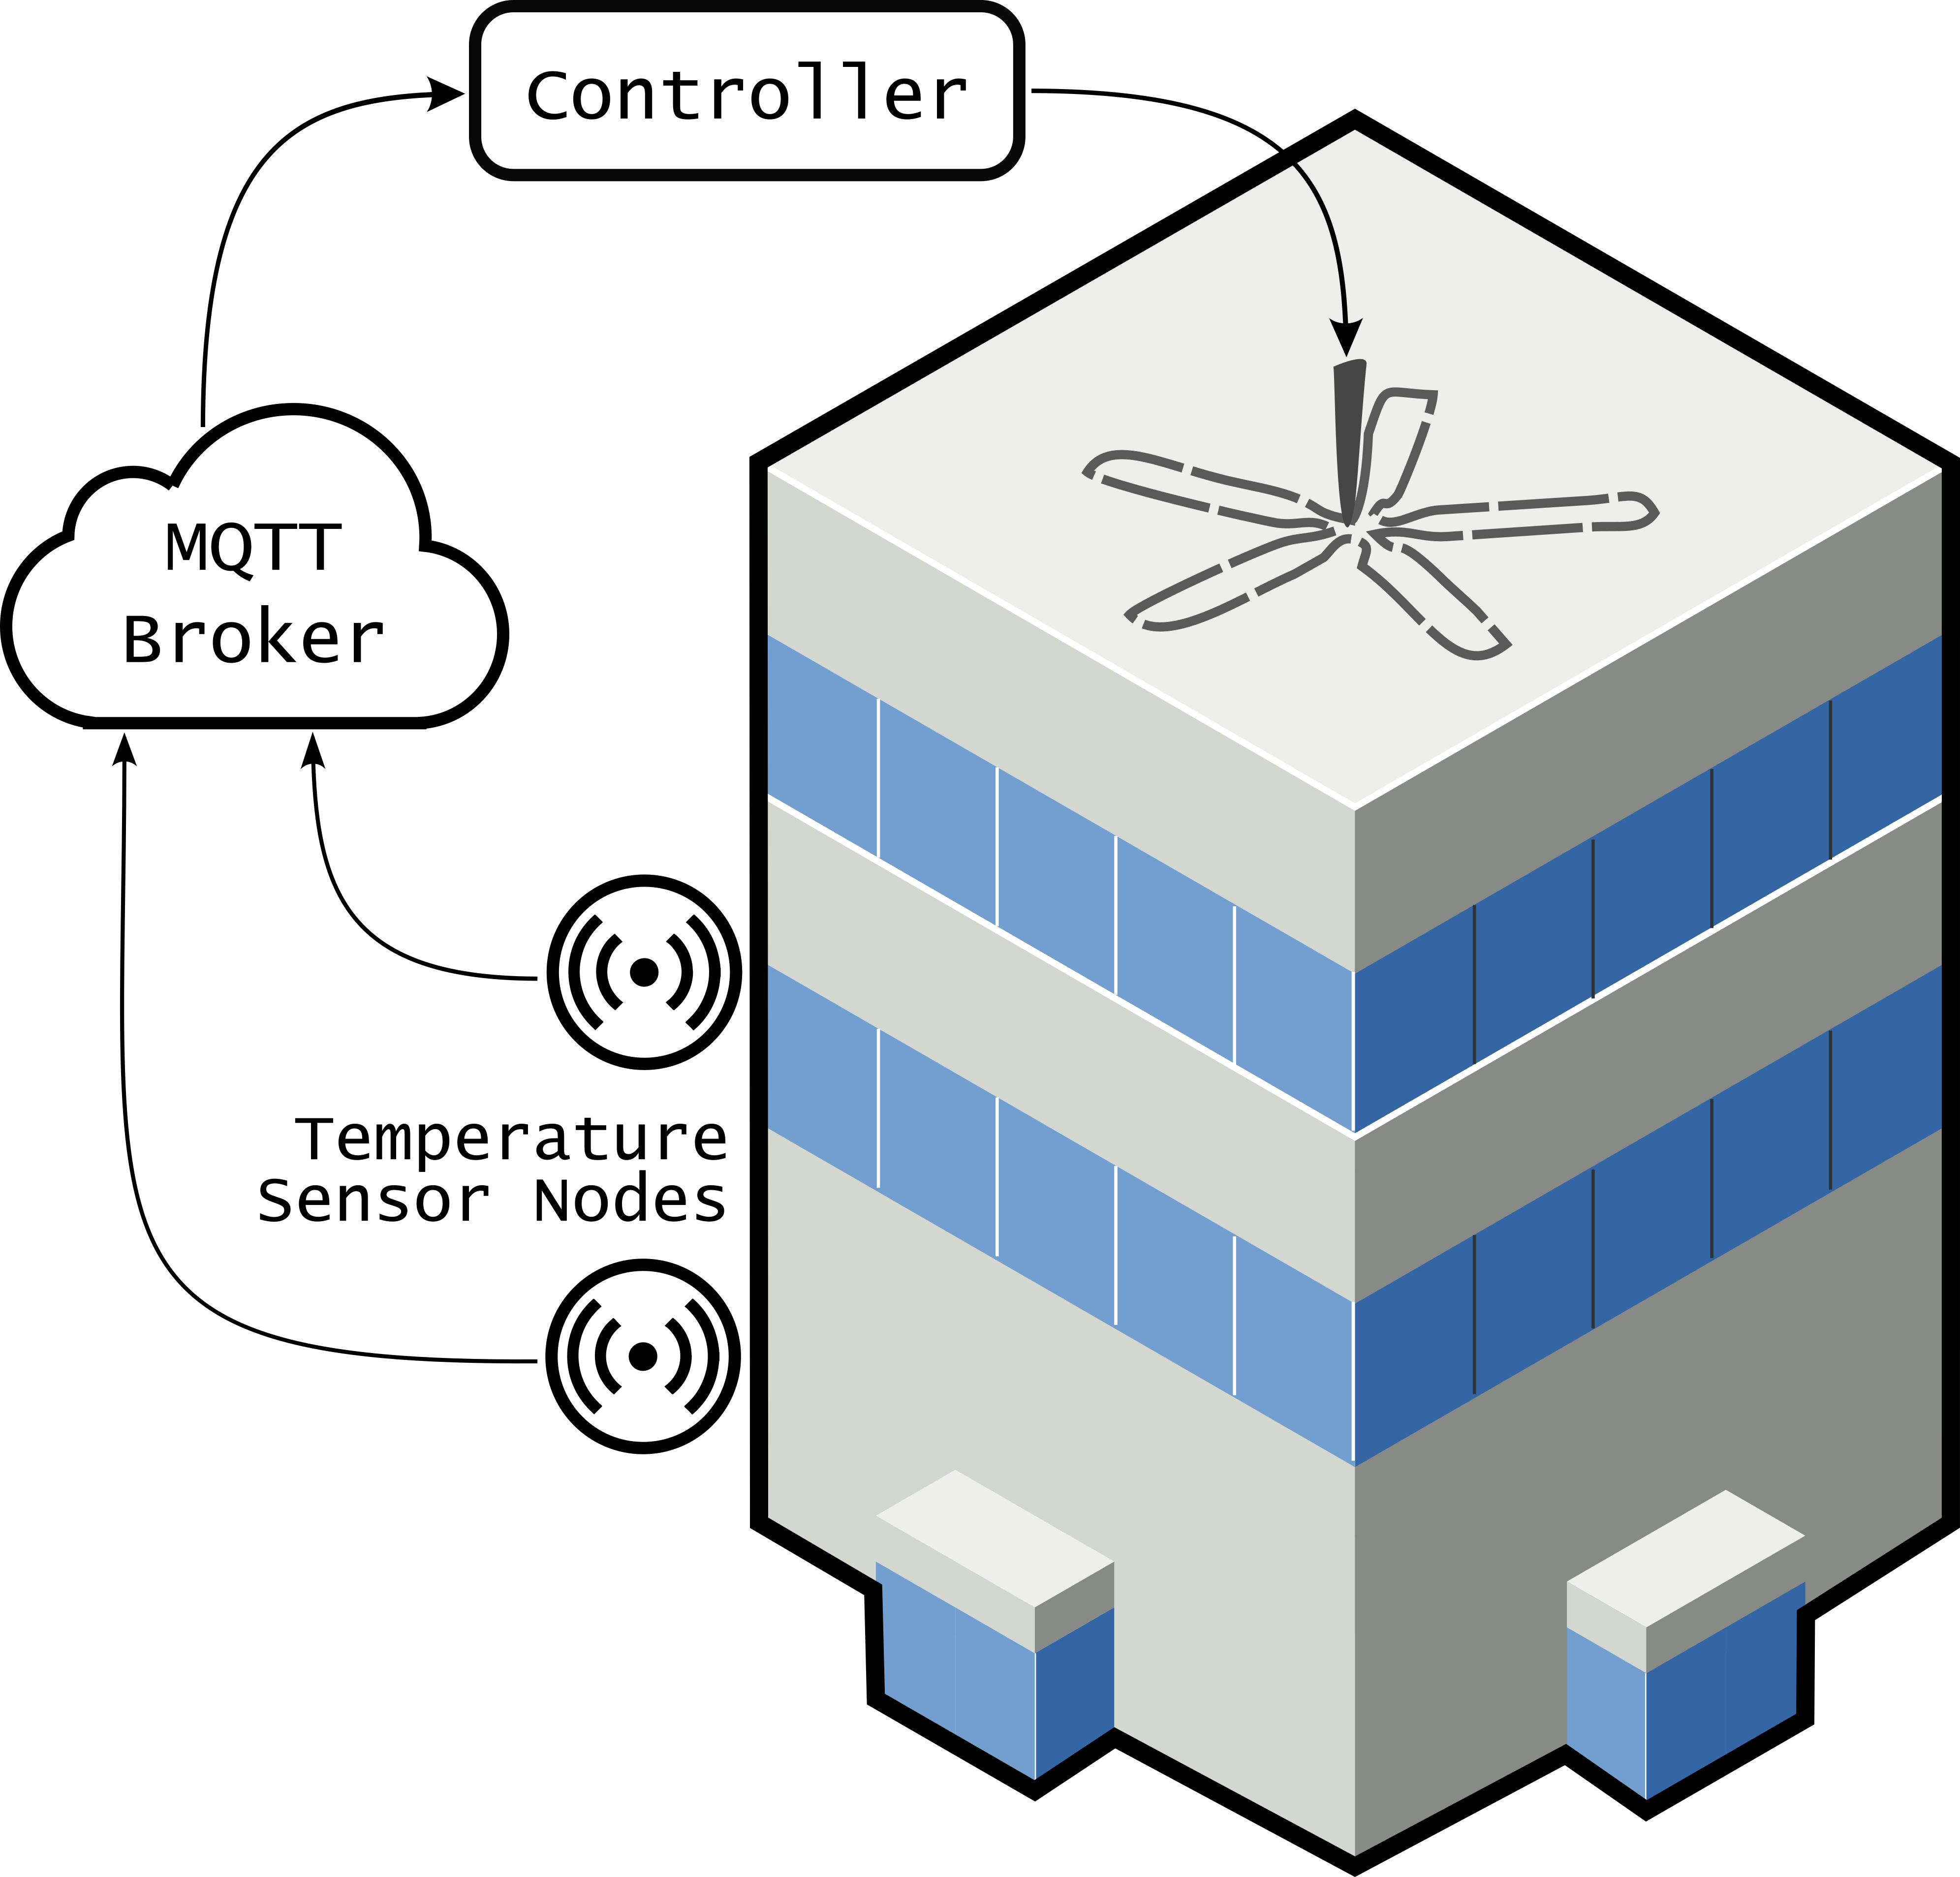
\includegraphics[width=0.5\textwidth]{img/overall-system}
								\caption{The Overall Temperature Measurement and Control System Diagram}
								\label{fig:overall-system}
							%\end{minipage}
%							\hspace{1em}
%							\begin{minipage}{0.45\textwidth}
%								\centering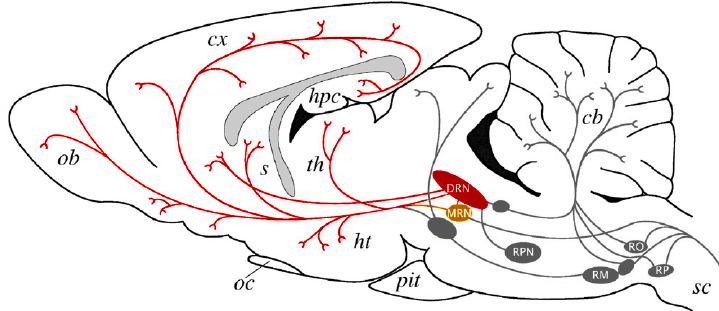
\includegraphics[width=1\textwidth]{img/drn_mr_p.png}
%								\caption{Ascending serotonergic projections alone innervate the majority of cortical and subcortical areas \cite{Oegren2008}}
%							\end{minipage}
						\end{figure}
					\end{myblock}	\vspace{.5cm}
				
					\begin{myblock}{Project Description}
						The aim of the project is to design and produce a autonomous vehicle that can follow a path with varying propoerties.
						
						Throughout the project we have followed an design methodology called Agile Methodology. Agile development approach relies on rapid development and prototype production. We have also divided the project into subsections according to V-model.
						
					\end{myblock}	\vspace{0.4em}
				
			
				\begin{myblock}{Project Specifications and Requirements}
					\begin{figure}
						\centering
						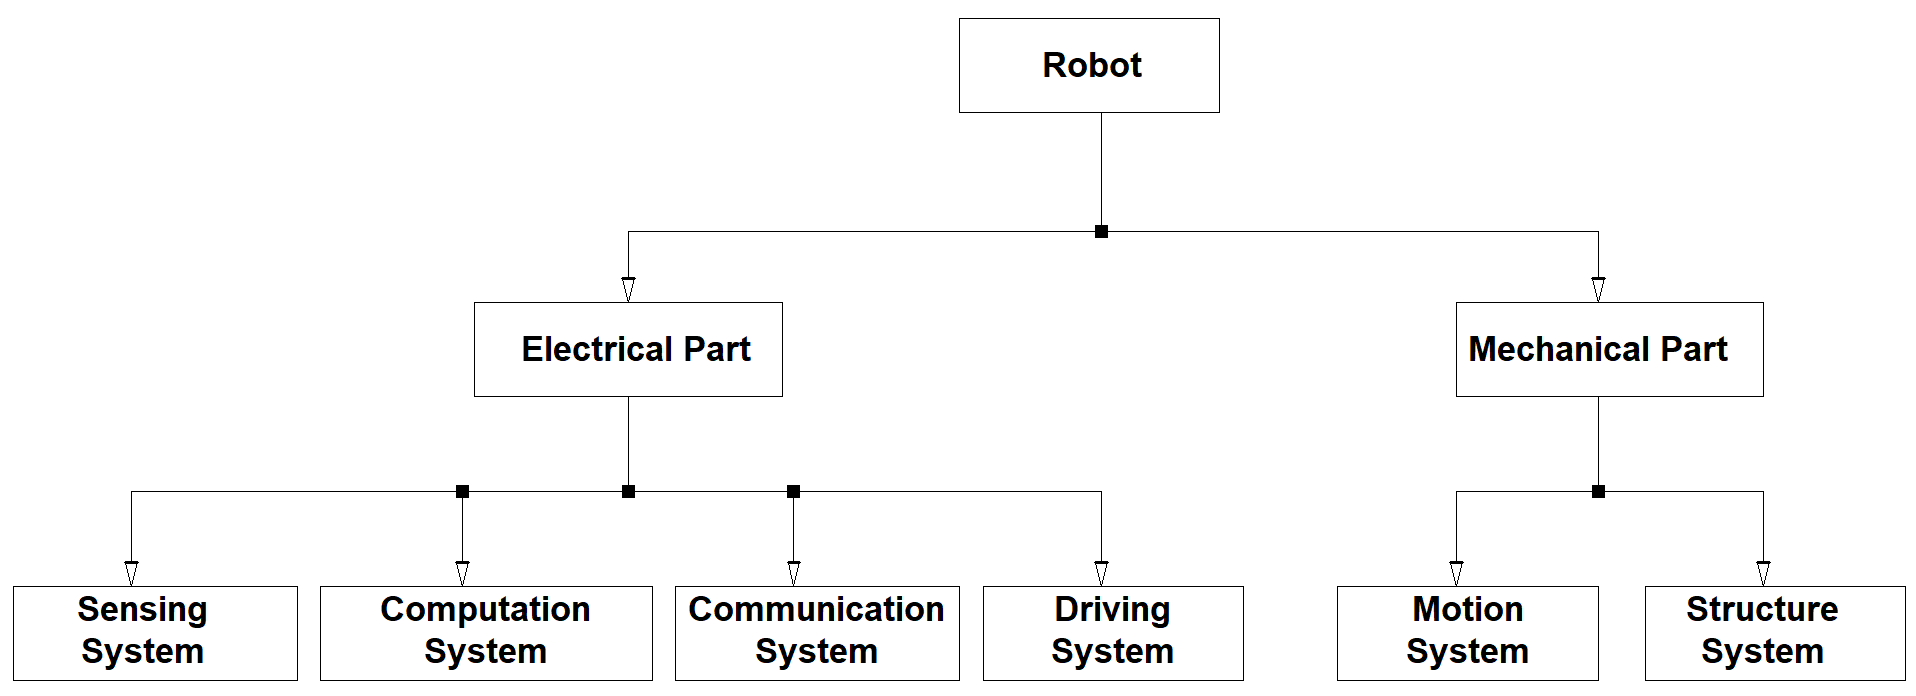
\includegraphics[width=\textwidth]{img/systems}
						\caption{System Diagram of the Project}
						\label{fig:overall-system}
					\end{figure}
				\vspace{1cm}
				\begin{table}
					\caption{Requirements of the Project}
					\begin{tabular}{ll}
						%\cline{1-2}
						Project Requirements   & System Requirement \\
						\hline 
						\multirow{2}{*}{Follow path in every condition }       &  SenS: Detect lane in varying conditions       \\
						&  CmpS: Eliminate obstacles \\
						\hline
						\multirow{2}{*}{Complete path within 15 seconds}    & CmpS: Produce consistent error signal  \\
						& CmpS: Have robust controller performance  \\
						\hline
						\multirow{2}{*}{Not crash to opponent}   & SenS: Detect opponent atmost at 5 cm        \\
						& CmpS: Not be affected by the opponent \\
						\hline
						\multirow{2}{*}{Communicate with opponents}  & \multirow{2}{*}{CmnS: Follow the Handshake Protocol}      \\
						& \\
						\hline
						\multirow{2}{*}{Battery life at least 1 hour} & StrS: Supply () mW power \\
						&  MtnS: Consume at max () mW \\
						\hline
						\multirow{2}{*}{Production price less than  $\$200$} & StrS: Pyhsical materials cost at most  $\$200$\\
						& MtnS: Cost less than $\$35$  \\
						\hline
					\end{tabular}
				\end{table}
	\end{myblock}	\vspace{0.4em}
	\begin{myblock}{Proposed Solution}
		d
	\end{myblock}	

		}\end{minipage}\end{beamercolorbox}
	\end{column}
	\begin{column}{.5\textwidth}
		\begin{beamercolorbox}[center]{postercolumn}
			\begin{minipage}{.98\textwidth} % tweaks the width, makes a new \textwidth
				\parbox[t][\columnheight]{\textwidth}{ % must be some better way to set the the height, width and textwidth simultaneously
					\begin{myblock}{Cost Breakdown}
				BB
					\end{myblock} \vfill
					\begin{myblock}{Deliverables}
				CC
					\end{myblock} \vfill
					\begin{myblock}{References}
						\footnotesize
						\bibliographystyle{ieeetr}
						\bibliography{./bib}
					\end{myblock}
		}\end{minipage}\end{beamercolorbox}
	\end{column}
\end{columns}
\end{frame}
\end{document}
